\documentclass[a4paper,12pt]{article} 
\usepackage{graphicx} % Required for inserting images
\usepackage{graphicx} % Required for inserting images
\usepackage{cmap}
\usepackage{mathtext}
\usepackage{amssymb}
\usepackage{amsmath}
\usepackage[russian]{babel}
\usepackage{indentfirst}
\usepackage[pdftex]{graphicx}
\usepackage{multirow}
\usepackage{siunitx}
\usepackage[left=2cm,right=2cm,top=2cm,bottom=2cm]{geometry}
\usepackage{fancyhdr}
\usepackage{float}

\usepackage[table]{xcolor}

\author{Егор Баранов, Шорина Анна}
\date{\today}

\begin{document}

\begin{center}
	\footnotesize{ФЕДЕРАЛЬНОЕ ГОСУДАРСТВЕННОЕ АВТОНОМНОЕ ОБРАЗОВАТЕЛЬНОЕ 	
    \\УЧРЕЖДЕНИЕ ВЫСШЕГО ОБРАЗОВАНИЯ}\\
	\footnotesize{МОСКОВСКИЙ ФИЗИКО-ТЕХНИЧЕСКИЙ ИНСТИТУТ\\(НАЦИОНАЛЬНЫЙ 			ИССЛЕДОВАТЕЛЬСКИЙ УНИВЕРСИТЕТ)}\\
	\hfill \break

	\hfill \break
	\hfill \break
	\hfill \break
	\hfill \break
	\hfill \break
	\hfill \break
	\hfill \break
	\hfill \break
	\Large{Лабораторная работа \\\textbf{Образование, устойчивость и свойства лиофобных коллоидных растворов}}\\
	\hfill \break
	\hfill \break
	\hfill \break
	\begin{flushright}
		Вернер Никита, Чекмарёв Игорь\\
		Группа Б06-404
	\end{flushright}
	\hfill \break
	\hfill \break
	\hfill \break
	\hfill \break
	\hfill \break
	\hfill \break
	\hfill \break
	\hfill \break
	\hfill \break
	\hfill \break
\end{center}
\begin{center}
	Долгопрудный, 2026
\end{center}
\thispagestyle{empty}
\newpage

\section{Цели и задачи}
\noindent \textbf{Целями} данной работы являются:
\begin{enumerate}
    \item Изучение различных методик получения лиофобных коллоидных растворов и исследование их характерных свойств;
    \item Определение порога быстрой коагуляции выбранного золя при воздействии различных электролитов.
\end{enumerate}
Для реализации целей были поставлены следующие \textbf{задачи}:
\begin{enumerate}
      \item Получить коллоидный раствор серы $S$ методом замены растворителя; коллоидный раствор гидроксида железа $Fe(OH)_3$ методами конденсации и пептизации, а также коллоидный раствор золота $Au$;
    \item Пронаблюдать характерные физические свойства коллоидных систем;
    \item Сравнить степень пептизации раствора $Fe(OH)_3$ при различном количестве добавленного пептизатора;
    \item Зарегистрировать спектр экстинкции золя золота $Au$, оценить размер наночастиц и их концентрацию; вычислить константу скорости быстрой коагуляции  и время, за которое количество исходных частиц уменьшается вдвое;
    \item Определить порог коагуляции золя золота $Au$ для различных электролитов.
\end{enumerate}

\section{Теоретическая справка}
Коллоидные растворы занимают промежуточное положение между истинными растворами и грубыми смесями (эмульсиями и суспензиями). Коллоидные растворы подразделяются на
\textit{лиофильные} и \textit{лиофобные}. Первые отличаются большим сродством к растворителю, являются термодинамически устойчивыми к агрегации и образуются самопроизвольно. Лиофобные коллоидные растворы, напротив, имеют низкое сродство к растворителю и представляют собой термодинамически неустойчивые к агрегации системы (из-за большого избытка поверхностной энергии); образуются в ходе конденсации из пересыщенного раствора  или несамопроизвольно в результате диспергирования. Однако такие системы могут быть устойчивы кинетически.

\subsection*{Кинетическая устойчивость лиофобных коллоидных систем}
В настоящее время выделяют три различных типа кинетических факторов устойчивости коллоидных растворов:
\begin{enumerate}
    \item Структурно-механический, обусловленный длительностью процесса разрушения упругих и прочных структур на поверхности диспергированных частиц;
    \item Гидродинамический, обусловленный снижением скорости частиц дисперсии при изменении вязкости и плотности дисперсионной среды;
    \item Смешанные, обусловленные действием нескольких кинетических факторов одновременно, что характерно для реальных cистем.
\end{enumerate}
Агрегативная устойчивость определяется скоростью процесса
коагуляции, описываемой моделью Смолуховского: 

\begin{equation}
    \frac{dn}{dt} = -kn^2.
    \label{1}
\end{equation}
где $k$ – константа скорости коагуляции, а $n=n(\tau)$ – суммарная концентрация частиц дисперсии ко времени $\tau$ с момента начала коагуляции.
Проинтегрировав, получаем:
\begin{equation}
    n(\tau) = \frac{n_0}{1+kn_0\tau},
    \label{2}
\end{equation}
где $n_0$ -- исходное число частиц.
Пренебрегая зависимостью $k$ от соотношения размеров сталкивающихся частиц и считая, что частота столкновения частиц лимитируется их диффузией, получим следующее выражение для константы скорости быстрой коагуляции:

\begin{equation}
    k_{\text{быстр}} = \frac{8k_BT}{3\eta}
    \label{3}
\end{equation}
где $\eta$ -- вязкость растворителя. Данная формула получена в предположении, что агрегация частиц происходит при каждой их встрече, то есть без энергетического барьера. Такая коагуляция считается быстрой.

Для времени полувревращения в такой реакции можно написать:
\begin{equation}
    \frac{n_0}{2} = \frac{n_0}{1+kn_0 \tau_{1/2}}
    \label{4}
\end{equation}
и тогда:
\begin{equation}
    \tau_{1/2} = \frac{1}{kn_0}
    \label{5}
\end{equation}

\subsection*{Энергия взаимодействия между частицами в коллоидном растворе}

Энергетическая устойчивость коллоидных растворов заключается в нахождении оптимума между энергией отталкивания и притяжения частиц дисперсии. Согласно теории Дерягина-Ландау-Фервея-Овербека (ДЛФО) общий график заивисимости энергии от расстояния между частицами (Рис. \ref{длфо}) представляет собой суперпозицию энергии дисперсионных взаимодействий, обусловленных силами Ван-дер-Ваальса ($u_{\text{ВдВ}} \sim -\frac{1}{h^2}$), и энергии отталкивания $u_{\text{ДЭС}}  \sim e^{-h/\lambda} $, где $\lambda  = \sqrt{\frac{\varepsilon \varepsilon_0RT}{2F^2I}}$.

\begin{figure}[H]
	\center{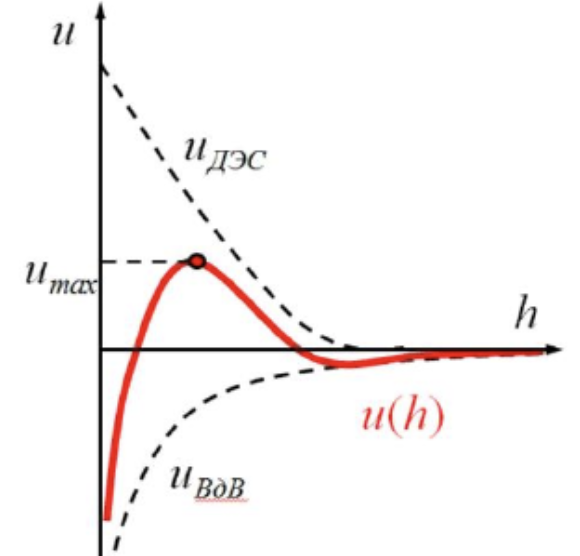
\includegraphics[scale=0.5]{длфо.png}}
	\caption{Зависимость энергии взаимодействия двух частиц от расстояния между ними}
    \label{длфо}
\end{figure}

Учитывая столь важную роль электростатических взаимодействий одним из наиболее известных способов коагуляции лиофобных систем является действие растворов электролитов. Согласно структуре двойного электрического слоя по действию на каждую из его составляющих различают два типа электролитной коагуляции:
\begin{itemize}
    \item Нейтрализационную (эффективна при низких поверхностных зарядах частиц), обусловленную понижением заряда диспергированных частиц за счет адсорбции на них противоионов;
    \item Концентрационную (эффективна при высоких поверхностных зарядах частиц), обусловленную сжатием двойного электрического слоя (при этом заряд поверхности не меняется).
\end{itemize}
Влияние электролитов на коагуляцию описывается правилом Шульце-Гарди: коагулирующим действием обладают те ионы электролита-коагулятора, знак заряда которых противоположен заряду частицы дисперсии, а коагулирующее действие возрастает с увеличением заряда иона-коагулятора. Для одно-, двух и трехвалентного ионов коагулирующее действие примерно относятся как 1: 50 : 500. 

Агрегации соответствует исчезновение потенциального барьера при введении некоторого определенного количества электролита. Необходимая для этого концентрация
электролита называется \textbf{порогом быстрой коагуляции}:
\begin{equation}
C_{\mbox{пк}} = \frac{C_{\mbox{э}}\cdot V_{\mbox{э}}}{V_{\mbox{з}} + V_{\mbox{э}}},    
\end{equation}
где $C_{\mbox{э}}$ и -- $V_{\mbox{э}}$ концентрация и объем добавленного электролита, $V_{\mbox{з}}$ -- объем золя.

Существует \textbf{правило Дерягина-Ландау}: при электролитной коагуляции по концентрационному механизму порог коагуляции обратно пропорционален заряду противоионов в шестой степени; а также  \textbf{правило Эйлерса-Корфа:} при нейтрализационной коагуляции порог коагуляции обратно пропорционален второй степени заряда добавляемых противоионов.

\subsection*{Строение мицелл лиофобных коллоидных растворов}
У коллоидных частиц поверхностный заряд обусловлен избирательной адсорбцией ионов, либо диссоциацией поверхностных групп. Возникающая заряженная частица, окруженная противоионами называется мицеллой, подобно мицеллам ПАВ.
\begin{figure}[H]
	\center{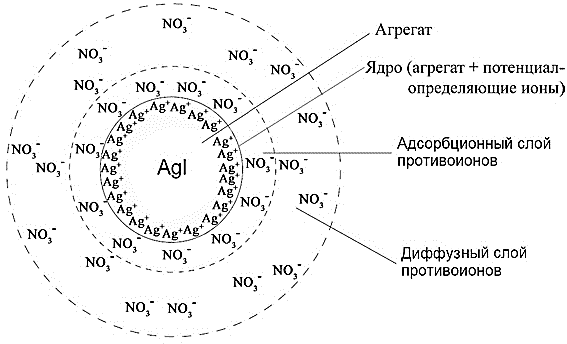
\includegraphics[scale=0.6]{2.png}}
	\caption{Пример строения коллоидной мицеллы}
\end{figure}
Как и у поверхности металлических электродов слой противоионов разделяют на две составляющие – плотную часть, в которой ионы находятся непосредственно у заряженной поверхности и диффузную часть, где нейтрализующий заряд постепенно спадает в глубь раствора. Одним из распространенных методов оценки заряда и потенциала коллоидных частиц является определение скорости их движения в электрическом поле. Однако в процессе такого движения двойной электрический слой разрывается. Место разрыва при перемещении твердой и жидкой фаз друг относительно друга называется плоскостью скольжения. Потенциал на плоскости скольжения называют электрокинетическим или дзета-потенциалом ($\zeta$ -потенциал). Другими словами, $\zeta$ -потенциал – это разность потенциалов в объеме дисперсионной среды и в плоскости скольжения, т.е. на границе неподвижного слоя жидкости, окружающего частицу. Важность $\zeta$ -потенциала состоит в том, что его значение может быть связано с устойчивостью коллоидных дисперсий. Обычно, устойчивым коллоидам соответствует значение $\zeta$ -потенциала, превышающее по абсолютной величине 30 мВ.

\section{Измерения и обработка результатов измерений}

\subsection*{1. Получение золя серы методом замены растворителя}
Нальем в пробирку около 5 мл дистиллированной воды и добавим 1 мл насыщенного раствора серы в ацетоне; перемешаем. Через некоторое время раствор начинает опалесцировать (при проходящем свете окрашивается в жёлтый, а при боковом - в голубоватый), что говорит об образовании золя серы. 

\begin{figure}[H]
	\centering
		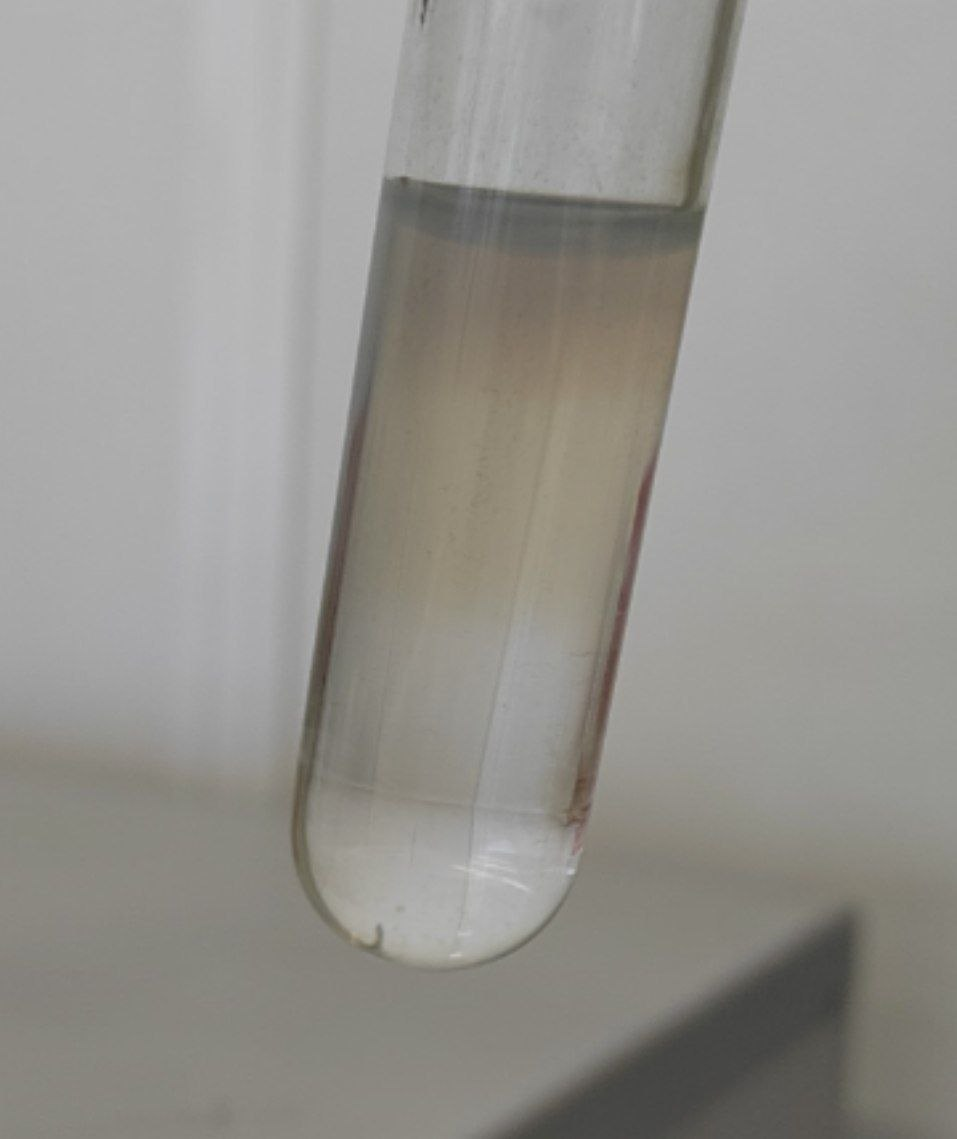
\includegraphics[width=0.3\linewidth]{сера 1.png}
	\caption{Полученный золь серы}
\end{figure}
\subsection*{2. Получение золя гидроксида железа методом конденсации (Методом Крекке)}
В закипевшую на магнитной мешалке воду мы добавляем 5мл 2\%-раствора $FeCl_3$. В результате наблюдаем образование раствора коньячного цвета. 

В результате происходят реакции:
\begin{equation*}
    FeCl_3+3H_20 \rightarrow Fe(OH)_3+3HCl
\end{equation*}
\begin{equation*}
    Fe(OH)_3+HCl \rightarrow FeOCl + 2H_2O
\end{equation*}
В итоге получается коллоидный раствор, в котором формула мицеллы золя выглядит так:
\begin{equation*}
    \{[mFe(OH)_3]nFeO^+ (n-x)Cl^-\}^{x+}xCl^-
\end{equation*}
По правилу Фаянсова-Пескова-Панета лучше будут адсорбироваться те ионы, которые достраивают кристаллическую решетку. В нашем растворе это $Fe^{3+}$ и $FeO^+$. В следствие того, что реакция протекает при высокой температуре, $Fe^{3+}$ оказывается в значительной степени гидролизован, значит в растворе преобладает $FeO^+$, следовательно, именно он и будет преимущественно адсорбироваться на поверхности мицеллы
\begin{figure}[H]
    \centering
    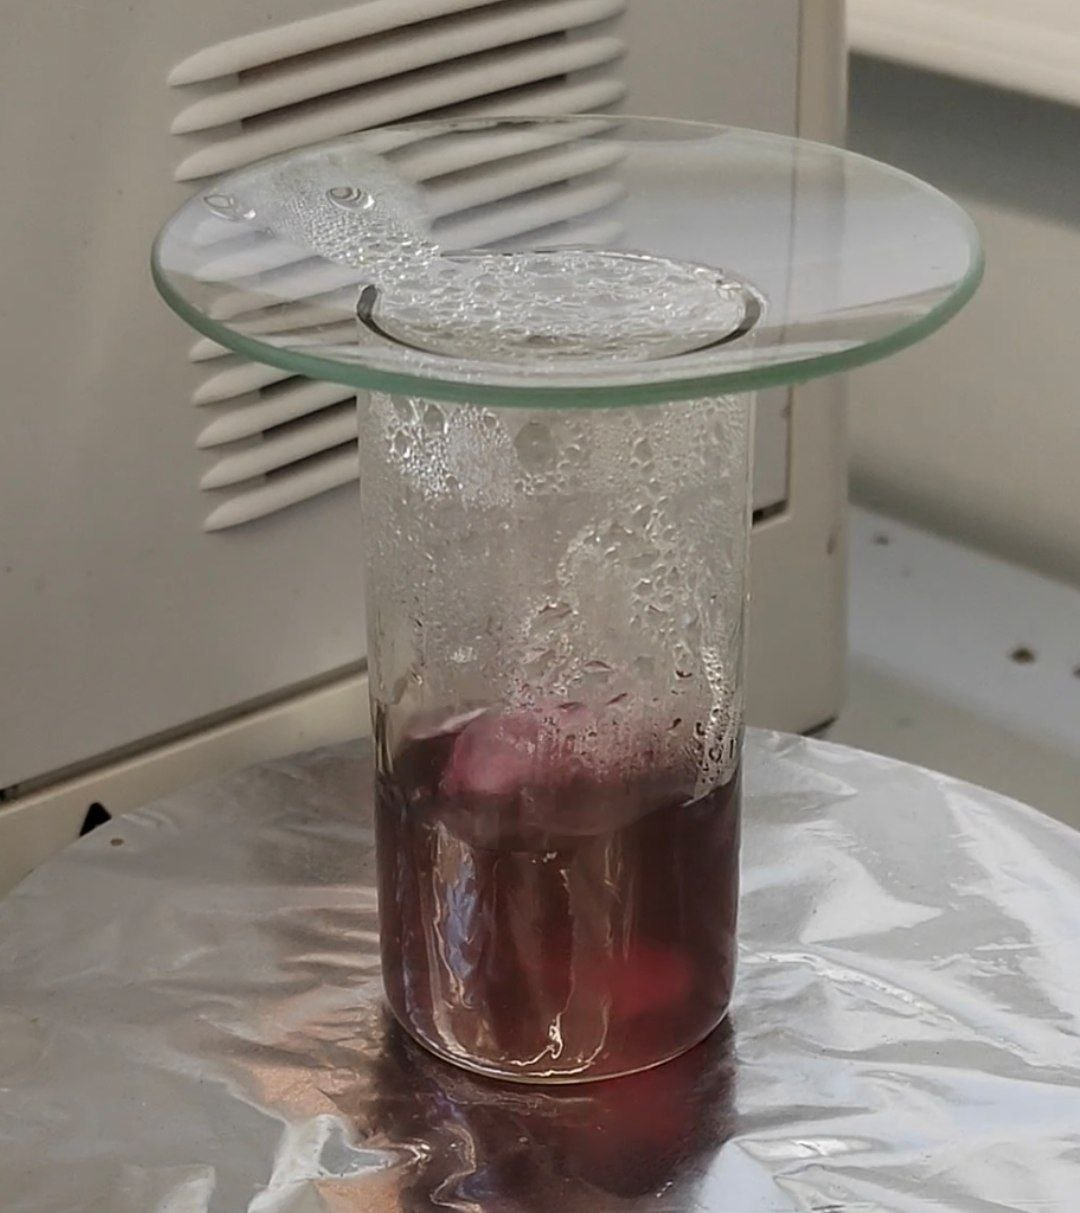
\includegraphics[width=0.5\linewidth]{коньяк.png}
    \caption{Полученный раствор}
    \label{fig:enter-label}
\end{figure}

\subsection*{3. Получение золя гидроксида железа методом пептизации}
\begin{figure}[H]
	\centering
		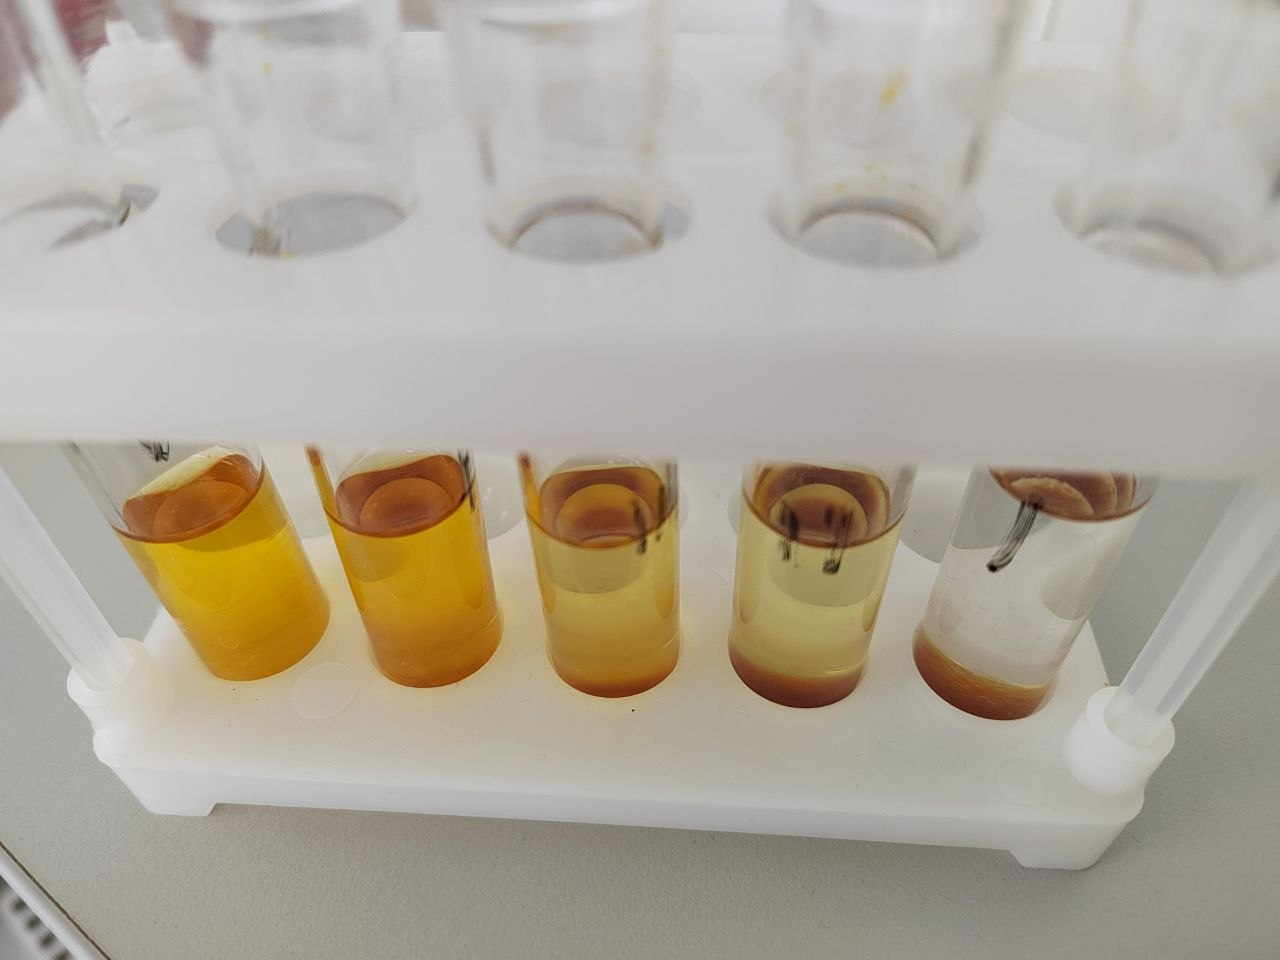
\includegraphics[width=0.3\linewidth]{image.png}
	\caption{Полученные растворы}
\end{figure}
 В стакан отмерим 25 мл дистиллированной воды и 0,5 мл 10$\%$-ного раствора $FeCl_3$. К полученному раствору по каплям добавим 5$\%$-ный раствор аммиака до тех пор, пока количество образующегося осадка не перестанет увеличиваться. В растворе происходит реакция:
    $$FeCl_3 + 3NH_3 \cdot H_2O \rightarrow Fe(OH)_3\downarrow + 3NH_4Cl$$

Дадим осадку полностью осесть, затем проведём три серии декантации с полученным раствором. К промытому осадку добавим 25 мл дистиллированной воды, взболтаем и, не давая гидроксиду железа осесть, перенесём пипеткой по 2 мл образовавшейся суспензии в 5 пробирок. В каждую из пробирок (кроме первой) добавим фиксированный объём 10$\%$-ного раствора $FeCl_3$ (выступает в качестве пептизатора). Энергично перемещаем содержимое и оставим пробирки в штативе на час. В растворах происходят процессы пептизации и образуются положительно заряженные коллоидные частицы:
    $$ mFe(OH)_3+nFeCl_3 \rightarrow \{[mFe(OH)_3]~nFe^{3+}~3(n-x)Cl^-\}^{3x+}~3xCl^-$$
По истечении часа сравним объемы осадков в пробирках с пептизатором и в контрольной пробирке (№ 1). Результаты занесем в таблицу \ref{пептизация}, отметив в нижней строке степень пептизации, используя символы: «--» – отсутствие пептизации, «+, ++, +++» -- частичная пептизация и «++++» -- полная пептизация.

\begin{table}[h!]
    \caption{Сравнение степени пептизации}
    \centering
    \label{пептизация}
\begin{tabular}{|l|l|l|l|l|l|}
\hline
№ пробирки & 1 & 2 & 3 & 4 & 5 \\ \hline
Объём суспензии, мл & 2 & 2 & 2 & 2 & 2 \\ \hline
Объём воды, мл & 5,0 & 4,8 & 4,6 & 4,4 & 4,2 \\ \hline
Объём 10-$\%$ $FeCl_3$, мл & 0 & 0,2 & 0,4 & 0,6 & 0,8 \\ \hline
Степень пептизации & - & + & ++ & +++ & ++++ \\ \hline
\end{tabular}
\end{table}

Можно видеть, что с увеличением объема добавленного раствора $FeCl_3$ степень пептизации возрастает, в результате чего гидроксид железа растворяется всё эффективнее. 

На поверхности $Fe(OH)_3$ преимущественно адсорбируются ионы $Fe^{3+}$, так как они способствуют достройке кристаллической решётки и обладают наибольшим зарядом среди присутствующих в системе ионов. Для полного перевода осадка $Fe(OH)_3$ в коллоидное состояние требуется 0,8 мл 10-$\%$-раствора  $FeCl_3$.

\subsection*{4. Получение золя золота методом Френса}
В 25мл дистиллированной воды, доведенной до кипения добавили 250мкл 1\%-раствора $HAuCl_4$. Через 3 минуты, когда кипение восстановилось, добавили 400мкл цитрата натрия. Раствор из прозрачного стал темно-синим, а затем плавно менял цвет до темно-красного. 

Образование золя золота происходит из-за реакции:
\begin{equation*}
    2HAuCl_4+3Na_3 ~ HOC(COO)(CH_2COO)_2 \rightarrow \newline 2Au +3Na_2~O=C(CH_2COO) + 3CO_2+3NaCl+5HCl
\end{equation*}

Определим исходные количества веществ:
\begin{equation*}
    \nu_{cit} = 1.55\cdot10^{-5}~моль
\end{equation*}
\begin{equation*}
    \nu_{Au} = 7.35\cdot10^{-6}~моль
\end{equation*}

Получается, что цитрат в избытке почти в 1.5 раза, значит, за место на поверхности конкурируют цитрат-ион и ионы натрия, но у цитрата больше заряд, поэтому золото оказывается стабилизировано цитратами.

Строение мицеллы золя:
 $$\{[mAu]nCyt^{3-}(3n-x)Na^{+}\}^{x-}xNa^{+}$$
Снимем спектр полученных наночастиц:
\begin{figure}[H]
    \centering
    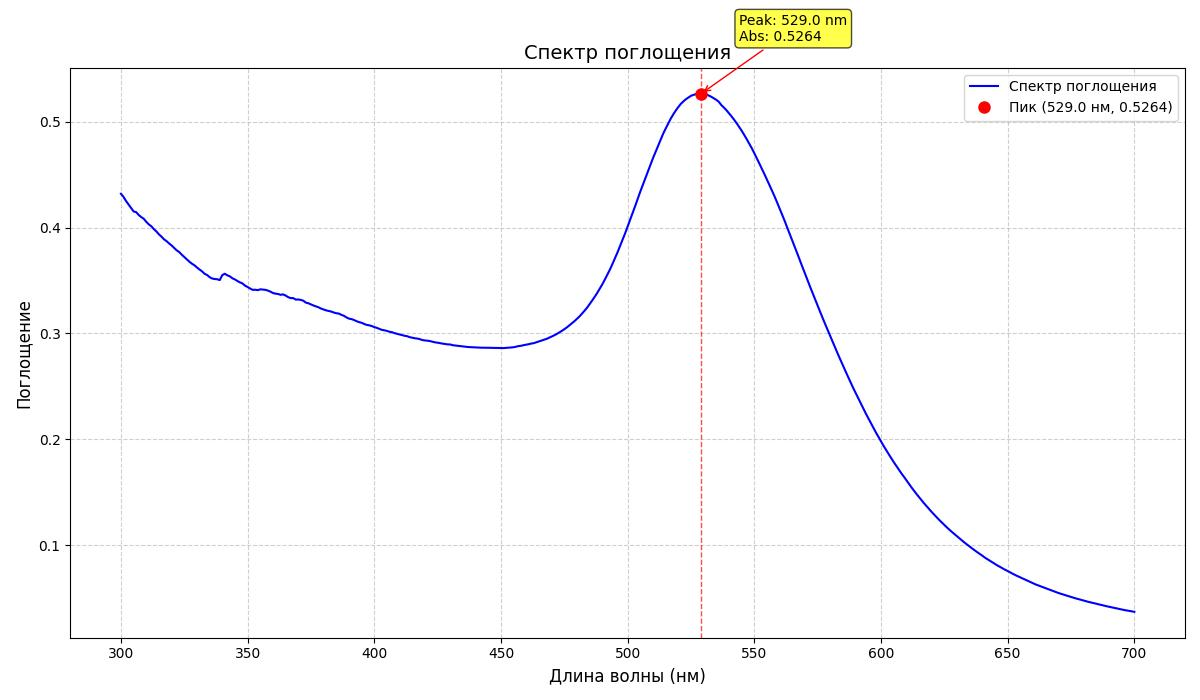
\includegraphics[width=1\linewidth]{abs_peak.jpg}
    \caption{Полученный спектр наночастиц золота}
    \label{fig:enter-label}
\end{figure}

\begin{figure}[H]
    \centering
    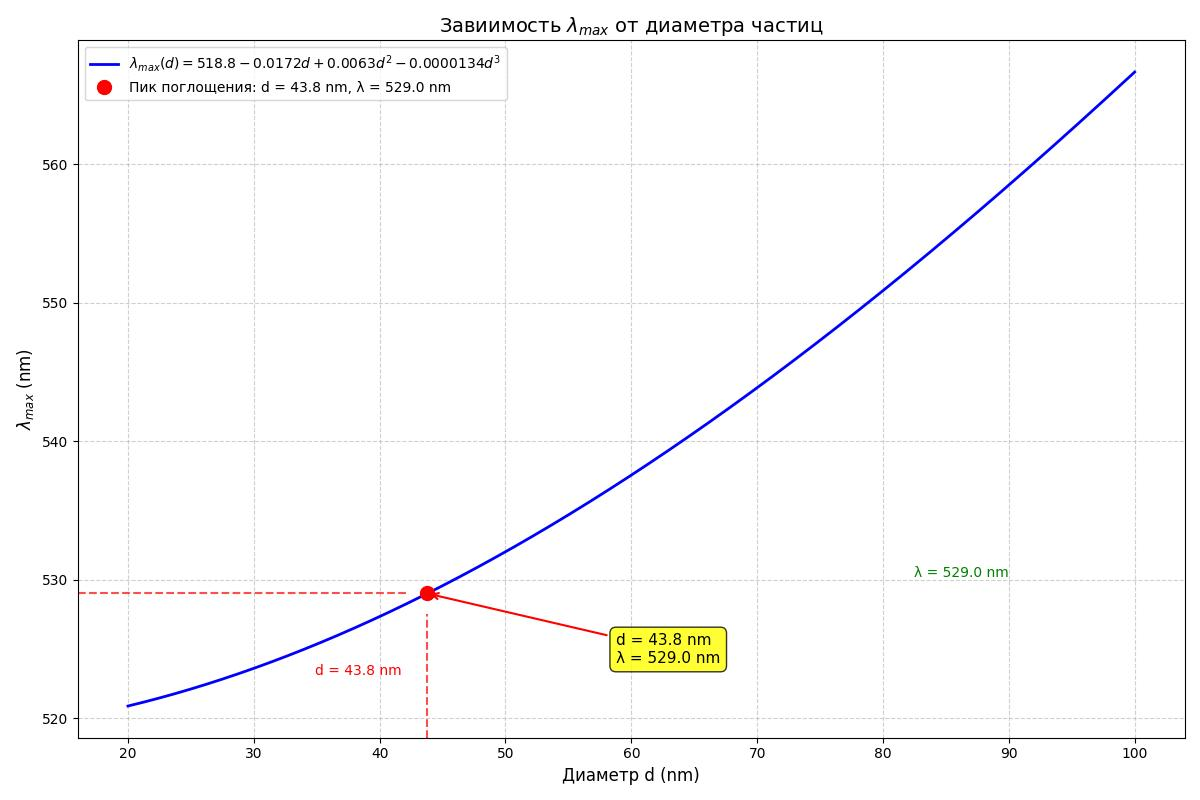
\includegraphics[width=1\linewidth]{lambda max.jpg}
    \caption{Соответствие пика поглощения размеру частиц}
    \label{fig:enter-label}
\end{figure}
Видим, что пик поглощения наблюдается при $\lambda = 529нм$, что соответствует размеру коллоидных частиц $\approx44~нм$.

Теперь определим концентрацию наночастиц. Считая, что частицы сферические и зная их диаметр, найдем количество атомов золота в одном агрегате:
\begin{equation*}
   N = \frac{\rho V N_a}{M_{Au}} = \frac{\pi d^3\rho N_a }{6M_{Au}} \approx 2650\cdot10^3
\end{equation*}
\begin{equation*}
    N_{np} = \frac{\nu_{Au}N_a}{N} = 1.67\cdot10^{12},
\end{equation*}
где $N$ -- число атомов золота в одной мицелле, $N_{np}$ -- число мицелл в растворе. Отсюда:
\begin{equation*}
    n_{np} = 2.27\cdot10^{17}~шт/м^3
\end{equation*}
Оценим константу скорости быстрой коагуляции по формуле (\ref{3}):
\begin{equation*}
    k_{быстр} = 1.23\cdot10^{-17}~м^3/c
\end{equation*}
Исходя из этого, оценим время полупревращения по (\ref{5}):
\begin{equation*}
    \tau_{1/2} = 0.36c
\end{equation*}

\subsection*{5.  Определение порога коагуляции золя золота}
Из формулы мицеллы золя следует, что золь обладает отрицательным зарядом, следовательно, его противоионами являются катионы.  

Для определения порога быстрой коагуляции необходимо установить такой объем добавляемого электролита, при котором изменение окраски происходит мгновенно. Измерения проводим следующим образом: в кювету наливаем 1 мл золя, затем добавляем определённое количество воды так, чтобы общий объем раствора составлял 3 мл. В конце вносим электролит и наблюдаем, произошло ли помутнение. Данные занесем в таблицу:

\begin{table}[H]
    \centering
    \begin{tabular}{|c|c|c|c|c|c|}
    \hline
        $V(KNO_3)$, мл & результат & $V(Mg(NO_3)_2)$, мл & результат & $V(La(NO_3)_3)$, мл & результат  \\ \hline
        2 & + & 0,5 & + & 0,5 & +  \\ \hline
        1 & + & 0,25 & + & 0,25 & +  \\ \hline
        0,5 & + & 0,125 & - & 0,125 & -  \\ \hline
        0,25 & + & 0,187 & + & \cellcolor{green!50}0,187 & +  \\ \hline
        0,125 & - & \cellcolor{green!50}0,156 & + & 0,156 & -  \\ \hline
        0,187 & - & ~ & ~ & ~ &   \\ \hline
        \cellcolor{green!50}0,2 & + & ~ & ~ & ~ &   \\ \hline
    \end{tabular}
    \caption{Протекание быстрой коагуляции от объема электролита}
\end{table}
\begin{table}[H]
    \centering
    \begin{tabular}{|c|c|c|}
    \hline
        $C_{\text{ПК}}(KNO_3)$, мМ & $C_{\text{ПК}}(Mg(NO_3)_2)$, мМ & $C_{\text{ПК}}(La(NO_3)_3)$, мМ \\ %\hline
        33 & 0,52 & 0,13 \\  \hline
    \end{tabular}
    \caption{Пороги коагуляции}
\end{table}
\begin{figure}[H]
    \centering
    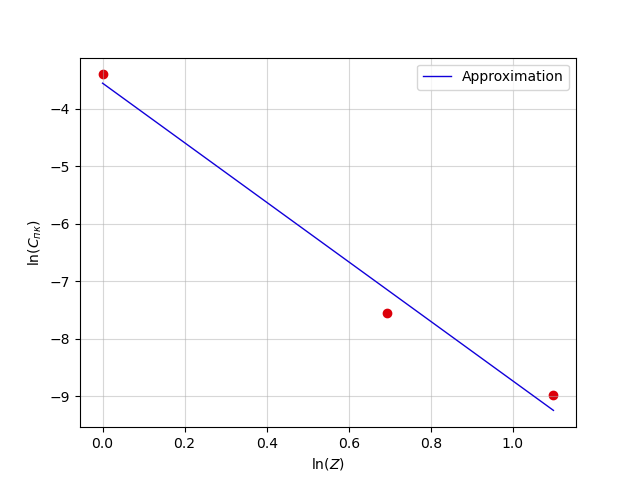
\includegraphics[width=0.7\linewidth]{graph.png}
    \caption{Зависимость логарифма C_{ПК} \hspace{1.5mm}от\hspace{1.5mm} логарифма \hspace{1.5mm}заряда\hspace{1.5mm} иона}
    \label{fig:enter-label}
\end{figure}

По графику получаем, что коэффициент перед ln(z) = -5.2, что говорит о том, что имеет место быть некоторое наложение теорий Дерягина-Ландау и Эйлерса-Корфа, однако первая описывает явление в опыте лучше.
\section{Выводы}

\begin{itemize}
\item В данной работе был получен колоидный раствор серы методом замены растворителя с менее полярного (ацетон) на более полярный (воду); зафиксировано явление опалесценции.
\item Был получен золь $Fe(OH)_3$ методом конденсации с помощью гидролиза раствора $FeCl_3$.
\item В ходе получения золя гидроксида железа $Fe(OH)_3$ методом пептизации была установлена зависимость степени пептизации от концентрации пептизатора $FeCl_3$.
\item Были синтезированы отрицательно заряженные коллоидные частицы золота методом Френса. Определен их размер по калибровочной кривой ($r\approx15~нм$), а также вычислена концентрация частиц в растворе ($n_{np} = 1.6\cdot10^{18}~шт/м^3$). Была оценена константа быстрой коагуляции $k_{быстр} = 1.23\cdot10^{-17}~м^3/c$, а также время полупревращения $\tau_{1/2} = 0.05c$.
\item Определены пороги коагуляции для ионов различных зарядов, построена линиаризованная зависимость $C_{ПК}(Z)$, найдено соотношение $C_{ПК}\sim Z^{-5.2}$, что говорит о протекании как концентрационной, так и нейтрализационной коагуляции.
\end{itemize}

\end{document}
\begin{figure}[H]
	\center{\includegraphics[scale=0.25]{пептизация.png}}
	\caption{Наглядное сравнение степени пептизации. Пробирки 1-5 (слева направо)}
    \label{пепт}
\end{figure}